\documentclass[12pt, a4paper]{report}

\usepackage{fyp}


%%these packages are not really necessary if you dont need the code and proofs environments
%%so if you like you can delete from here till the next comment
%%note that there are some examples below which obviously won't work once you remove this part
\usepackage{verbatim}
\usepackage{amsfonts}
\usepackage{amsmath}
\usepackage{amssymb}
\usepackage{amsthm}

\usepackage{pdfpages}
\usepackage{amssymb}
\usepackage{graphicx}
\usepackage{listings}
\usepackage{proof}
\usepackage{xcolor}
\usepackage{titlesec}
\usepackage{rotating}
\usepackage{float}
\usepackage{tikz}

\lstdefinelanguage{JavaScript}{
  keywords={typeof, new, true, false, catch, function, return, null, catch, switch, let, const, if, in, while, do, else, case, break},
  keywordstyle=\color{blue}\bfseries,
  ndkeywords={class, export, boolean, throw, implements, import, this},
  ndkeywordstyle=\color{darkgray}\bfseries,
  identifierstyle=\color{black},
  sensitive=false,
  comment=[l]{//},
  morecomment=[s]{/*}{*/},
  commentstyle=\color{purple}\ttfamily,
  stringstyle=\color{red}\ttfamily,
  morestring=[b]',
  morestring=[b]
}

\lstset{frame=tb,
  language=Python,
  aboveskip=3mm,
  belowskip=3mm,
  showstringspaces=false,
  columns=flexible,
  basicstyle={\small\ttfamily},
  numbers=none,
  numberstyle=\tiny\color{gray},
  keywordstyle=\color{blue},
  commentstyle=\color{dkgreen},
  stringstyle=\color{purple},
  breaklines=true,
  breakatwhitespace=true,
  tabsize=3,
  numbers=left
}

%%the following environments are useful to present proofs in your thesis
\theoremstyle{definition}
\newtheorem{definition}{Definition}[section]
\theoremstyle{definition}%plain}
\newtheorem{example}{Example}[section]
\theoremstyle{definition}%remark}
\newtheorem{proposition}{Proposition}[section]
\theoremstyle{definition}%remark}
\newtheorem{lemma}{Lemma}[section]
\theoremstyle{definition}%remark}
\newtheorem{corollary}{Corollary}[section]
\theoremstyle{definition}%remark}
\newtheorem{theorem}{Theorem}[section]
%%you can delete till here if you dont need the code and proofs environments



\setlength{\headheight}{15pt}
%\overfullrule=15pt


\begin{document}



%%make sure to enter this information
\title{JavaScript Framework for Actor-Based Programming}
\author{Andrew Buhagiar}
\date{\today}
\supervisor{Prof. Kevin Vella}
\department{Faculty of ICT}
\universitycrestpath{crest}
\submitdate{May 20, 2022} 

\frontmatter


\begin{acknowledgements}
your acknowledgements
\end{acknowledgements}
       
\begin{abstract}
an abstract
\end{abstract}

\tableofcontents

\listoffigures

\listoftables



\mainmatter

\chapter{Introduction}
\section{Motivation}
%Why JavaScript
JavaScript~\cite{ecmascript} is widely used for client applications on the browser and benefits from a growing popularity of server-side applications using environments such as Node.js. It is a single threaded language which lacks an intuitive way to program in a parallel and distributed fashion. This dissertation presents a prototype that implements a JavaScript framework which allows developers to build actor-based systems. Developers can use actors as concurrent units of computation which can be deployed either locally or remotely on multiple node runtimes and browsers. This will allow developers to intuitively distribute work amongst multiple processors and devices to fully utilise the hardware usually available in servers and modern computers.

%Why Actors
Actors~\cite{hewitt1973session}\cite{43years} communicate with each other through messages which are stored in the receiving actor's message queue. A message is processed by executing its defined actor behaviour. The Actor Model is a good fit for JavaScript's event loop~\cite{eventloopbrowser}\cite{eventloopnode} since they are both event driven. The Actor Model has already achieved success in the telecommunications industry and is more recently used for implementing distributed systems in languages such as Erlang and Scala/Akka~\cite{haller2012integration}.

\section{Objectives}
This dissertation will explore the suitability of the Actor Model when used to reason about distributed and concurrent systems in JavaScript through the use of one or multiple prototypes. The framework's suitability is based on its performance, scalablity, and intuitiveness to use. The objectives of the artifact are as follows.
\begin{enumerate}
    \item Allow developers to easily define and spawn actors through the framework API on Node.js or a browser. Actors should be able to send messages to other actors as well as spawn more actors. Full interoperability should be offered when using the framework across the two environments.
    \item Allow for spawning and interacting with actors on different Node.js processes through different network links. Node.js cluster\cite{cluster} can be used for IPC between node processes, while WebWorkers\cite{webworkers} can be used for communication between the primary thread and its spawned workers. When such communicaiton links are not available, the network stack is involved by using WebSockets for flexible communication to link remote processes and devices.
    \item Provide location transparency when dealing with actor references. Interacting with a local actor should be the same as interacting with a remote actor when using the API
    \item Benchmark the performance and scalability of the developed prototype.
\end{enumerate}

\chapter{Background}
\section{Concurrency and Parallelism on JavaScript}
Concurrency allows one to switch the order of the execution of tasks without yielding an incorrect output. Since the order in which a program is executed would not an issue, one can run these code segments in parallel, reducing the time taken to solve a particular problem. JavaScript and Node.js rely on a single threaded non-blocking event loop~\cite{eventloopbrowser}\cite{eventloopnode} which do not support parallel execution of such tasks, raising an issue when high performance~\cite{highperformance} computing is required. If JavaScript had to block when input or output was required, it would stop a page from being responsive. Instead, JavaScript handles I/O using events and callbacks which were posted on the event queue. The runtime will eventually process all the messages in a FIFO order, where each event has a corresponding callback or event listener function to execute. Each message is processed to completion without pre-emption by the processing of a different message, allowing for predictable concurrency of code. Web Workers\cite{webworkers} and child processes\cite{cluster} can be used to bring parallel computation to JavaScript~\cite{concurrencyjs}\cite{spidersjs} and uses a similar philosophy to that of the actor model. Both involve independently running tasks which communicate through messaging in order to allow for collaboration in solving a particular problem.

JavaScript is an implementation of the ECMAScript design. The ECMA-262 (ECMAScript 2021) language has multiple published editions, each of which serving as the blueprint for JavaScript’s next stable release. ECMAScript 8 provides the SharedArrayBuffer~\cite{es8}\cite{sharedarraybuffer} constructor which allows for concurrent access for a set of bytes. This allows for memory to be shared across agents in different cluster processes or webworkers. The process which created the SharedArrayBuffer need only pass the object to the workers to allow them to access and manipulate the same data block. SharedArrayBuffers allow for different workers to have access to the same memory which promotes collaboration when working on the same data points. However, parallel code accessing the same data may lead to data races and additional care must be taken by the developer.

\section{The History of the Actor Model}
The Actor Model was first introduced by Carl Hewitt~\cite{hewitt1973session}\cite{43years} in 1973 for research in artificial intelligence. It defines actors as computational agents which execute a uniform behaviour when sent a message. Hewitt argued that the actor metaphor can be applied to processes and daemons amongst other things. Two years later, Carl Hewitt helped in writing a draft of PLASMA, the first Actor Model language. In this language, actors communicate with each other using messages. The receiver processes the received message using its pre-defined computation. Based on the message’s contents, the actor may choose one from different behaviours which may involve sending messages to other actors.

The Actor Model was simplified by Gul Agha~\cite{agha1985actors} in 1986. While Carl Hewitt set the foundation of the potential applications of the actor metaphor, Gul Agha focused on how actors can be used to create expressive, simple, and intuitive programming languages. Gul Agha believed that it is more cost effective to use many smaller processors rather than rely on an individual powerful processor. His paper focused on the linguistic issues of a programming language which made concurrency intuitive when reasoning about collaborating processors. Gul Agha identified actors as computational agents which map incoming messages to a behaviour. Such behaviour may include communicating with other actors, deciding how the next incoming communication will be processed as well as creating more actors. He favoured buffered asynchronous communication when it came to sending messages as it allows an actor to communicate with itself without waiting, as well as to promote efficient use of the processing power rather than wait for the receiver to accept communication. Gul Agha also recognised the fact that delivery of messages is not guaranteed on a network, and that all receiving buffers are bounded.

In the same year as Gul Agha’s paper got released, a programming language called Erlang~\cite{erlang} made its first appearance. It was designed to address the highly concurrent nature of telephony applications. A high degree of fault tolerance was at the core of Erlang’s design to minimise failure in telephone systems when changing the system’s software. Erlang uses the actor model to allow for concurrent programming, such that each independent process communicates with other processes through the sending of messages. This makes “actors” and Erlang’s lightweight “processes” interchangeable in the remaining discussion of Erlang. Each process has a FIFO mailbox (queue) which processes the messages in the order they were received. Erlang adopts asynchronous message passing, promoting developers to “fire and forget” messages. The language is also designed to let processes crash, as external processes can easily observe each other. When a process which provides the service crashes, the monitoring process can take over and resume the service. Erlang was continuously updated and found success in large scale mobile networks thanks to the actor model’s potential to build reactive systems\cite{reactivemanifesto}. Erlang processes allow for elastic systems such that one can add more processes to address a larger workload, while monitoring processes allows for fault tolerance and responsiveness of the system. 

Nowadays, several variants of the actor model are used to fit the requirements of modern languages and frameworks. Popular languages such as Scala~\cite{scala} with Akka~\cite{akka} and Elixir~\cite{elixir} (built on top of Erlang) use the actor model to allow developers to build scalable and distributed systems.

\section{Similar Work}
Several JavaScript frameworks which implement the Actor model are already available on the node package manager (npm) and in public git repositories.

Clooney~\cite{clooney} is described as an actor library for the browser by the Google Chrome team. It offers an API that takes in classes with functions inside which will be instantiated in a worker. Developers can call the defined functions inside the actors as if they were a regular class. This library acts more as an intuitive way around using the Web Worker API to offer parallelism rather than a fully fledged actor library. 

Nact~\cite{nact} is a more faithful implementation to the Actor model as it relies on message passing for communication between isolated actors rather than Clooney's function calls. One spawns an actor by defining a function with the state, message and system context as the parameters. The function will be called for every message that is sent to the spawned actor. Network transparency has not been implemented for nact, making it more complex to have actors spawned on remote devices over the internet.

\textbf{Akka.js}~\cite{stivan2015akka} allows developers to cross-compile Akka to JavaScript browsers and server-side runtimes. This framework allows developers to build distributed applications using separate browsers using WebRTC~. It also incentivises developers to only be knowledgeable with Scala to deploy actors on both the browser and the server.

A project similar to this dissertation's prototype is called \textbf{Spiders.js}~\cite{spidersjs}. The paper identifies the problem of different API's being used for web workers and child processes, both of which are inspired by the actor model for constructing parallel systems using JavaScript. This project is focused on defining a single actor model API no matter if it's a client or server-side application. The paper benchmarks the usage of Spiders.js against JavaScript native web workers as well as the actor creation overhead for both. The results are in favour of using web workers for such tasks. This is no surprise as the project is an abstraction built on top web workers on the client side.

TigerQuoll~\cite{tigerquoll} took a different approach when providing parallelism to the language. It acknowledged the actor model as too limited for the requirements of more complex patterns that occur in modern applications. Instead it allows developers to use regular event based programming to register events for parallel processing. Other popular implementations on GitHub are Drama~\cite{drama} and Comedy~\cite{comedy}, both of which allow for sending messages to spawned actors. The latter implementation allows for spawning of actors on remote machines.
\chapter{Design}
The design chapter is split into three sections. The first section presents a high level overview of the API's features. The following section presents examples on how to use the framework's features through the use of code segments and explanations. The final section delves into the design decisions of the internal framework code which is abstracted by the API.
\section{API Features}
The API’s goal is to allow developers to intuitively engineer concurrent and parallel code in JavaScript through the actor model. The developer can define how an actor will process each message using a callback function, and spawn it on a JavaScript runtime. This runtime can be either local or remote, and it can run on a Node.js instance or any modern browser with full interoperability. Programs will be made up of multiple spawned isolated actors, similar to the micro-services approach adopted by the industry. Each actor will be serving incoming requests (messages) and can optionally send messages to other actors such as the sender. Furthermore, an actor can spawn other actors and send the reference to the newly spawned actors to other actors embedded inside a message.

\begin{figure}[H]
    \begin{centering}
        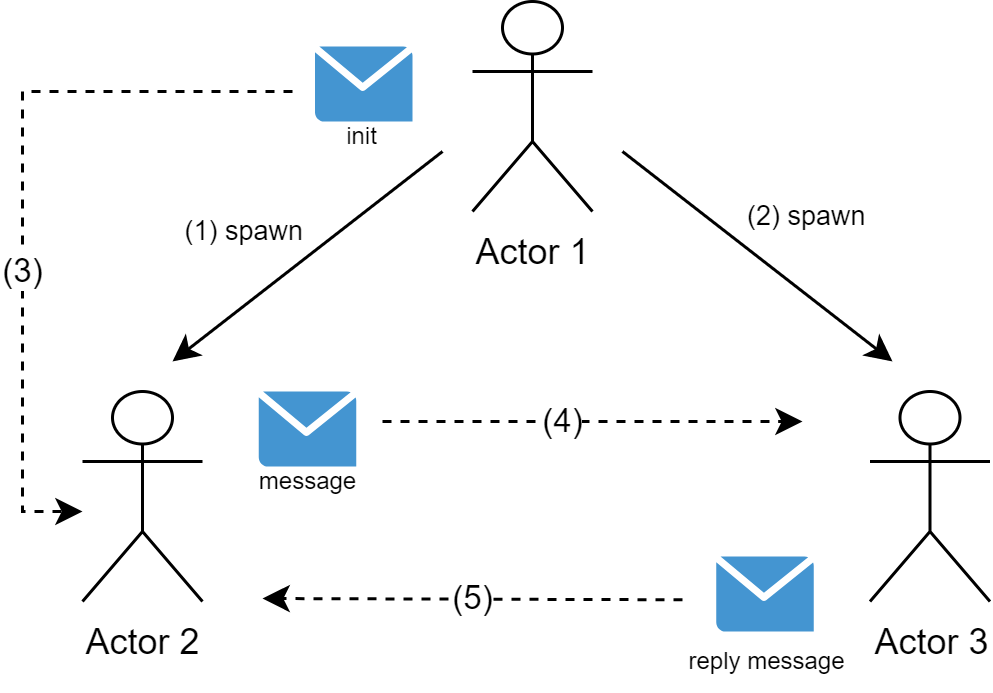
\includegraphics[width=250px]{resources/actors.png}
        \caption{Actor spawning a set of communicating Actors with labelled order}
    \end{centering}
\end{figure}

By sending messages to locally spawned actors, each message will be processed to completion in a FIFO order. Actors differ from regular functions as each spawned actor maintains a state which can be manipulated by its defined behaviour when executed in response to incoming messages. The actor’s behaviour can depend on the incoming message’s structure or the actor’s current state, offering seemingly non-uniform behaviour across messages. An actor can then be terminated where it will stop listening for incoming messages.

Since the spawned actors are isolated computational units, they are concurrent and thus potentially parallelisable. This API offers a mechanism to remotely spawn actors on other processes (shared memory) as well as over the web (distributed memory). One could host a website which remotely spawns actors on visiting clients to help speed up a computationally intensive task such as finding the next prime number. The more traction the website gains, the more computational power available.

Providing an intuitive way to remotely spawn and send messages to actors proved to be challenging. The prototype offers a WebSocket server which accepts a predefined number of clients. Each client is assigned a number, and when the number of expected clients connect the server sends a ‘ready’ message to all clients. This releases the barrier which waited for all clients to connect and allows communication between any two connected clients.

With the current implementation, the developer needs to connect the clients in a certain order to keep track of their incremental network numbers. The network number can then be used to indicate to the WebSocket server which client to communicate with. This is done when remotely spawning actors, as the developer needs to indicate on which connected client the actor will be spawned. Location transparency is offered when sending messages to such remotely spawned actors, as all the information required to establish communication is embedded within the actor reference. The API also allows the developer to make use of Node.js Cluster as well as Web Workers for faster communication, as it avoids adding the network stack and the overhead introduced when communicating with a potentially remote WebSocket server. All Node.js child processes and spawned web workers still need to establish a connection with the WebSocket server so that they are discoverable by remote devices.
\section{Using the API}
This section explores each of the functions that the framework exposes which developers will interact with to make use of the Actor Model in JavaScript. Using ES6 Modules the functions are imported as follows.
\begin{lstlisting}
import actors from './actors.js';
const { init, spawn, spawnRemote, terminate, send} = actors
\end{lstlisting}
\subsection{Spawning Local Actors}
When the developer calls the \textbf{spawn} function, they will pass in the actor's initial state as the first parameter. The actor will maintain this state throughout every processed message and it can be manipulated by its behaviour. The actor's state allows for it to maintain memory throughout its lifetime when processing messages. As a second parameter the developer must specify the actor's behaviour which has the actor's current state, current processed message as well as the actor's self reference as parameters. Using these parameters, the developer can define how the behaviour should manipulate the actor's state or how the message contents should be processed. It also allows the actor to pass a reference of itself to other actors using the behaviour's third parameter.

The example below defines the actor behaviour to print out each of the parameters. It then uses this function to spawn an actor with that behaviour, and a reference to that actor is returned
\begin{lstlisting}
//Actor behaviour
const pongBehaviour = (state, message, self) => {
    console.log("My state object is " + state);
    console.log("I'm processing the message object " + message);
    console.log("Actor self reference " + self);
};

//Spawn an actor with the above behaviour and an initial state
const pongReference = spawn({stateElement: "hello"}, pongBehaviour);
\end{lstlisting}
Note that with this implementation nothing is printed out, as the actor behaviour is only executed in response to a message which is sent to the spawned actor.
\subsection{Sending Messages to Actors}
The \textbf{send} function is used to send a message to an actor. It takes in the actor reference and message object to send as parameters.
\begin{lstlisting}
send(pongReference, {messageVal: "This is a message!"});
\end{lstlisting}
One of the framework's key features is location transparency. Whether the actor resides locally or remotely on a different process or device, the framework internally identifies the fastest medium to use for message transportation and sends it through that link.
\subsection{Terminating Actors}
An actor can be terminated using the \textbf{terminate} function. The function takes in the actor to terminate as the first parameter. An actor is terminated by removing its message listener as well as the internal record of the actor. The actor will however process its remaining messages as these are events already queued in the browser or Node.js's event loop. To forcefully terminate an actor, the second parameter can be set to true which will deactivate the actor. When the events are processed, the actor will perform minimal work ignoring the messages.
\begin{lstlisting}
terminate(pongReference, false)
\end{lstlisting}
\subsection{Connecting Processes to the Network}
The \textbf{init} function handles the spawning of worker processes as well as connections with other Node.js and browser runtimes through WebSockets.
\begin{lstlisting}
const webSocketServer = 'ws://localhost:8080';
const timeout = 10000;
const numberOfWorkers = 4;

init(webSocketServer, timeout, numberOfWorkers).then(ready => {
    if (ready.yourNetworkNumber === 1) {
        //Code for node 1 to execute
    }
})
\end{lstlisting}
 
\subsubsection{WebSocket Network}
Separate from the actor framework implementation, the prototype includes a WebSocket server implementation which handles a fixed number of expected WebSocket connections. As Node.js or browser runtimes connect to the WebSocket server through the invocation of \textbf{init}, the WebSocket server replies with acknowledgements. When the number of expected WebSocket connections are met, the server broadcasts to all connected clients that it is ready to receive and forward information. This effectively turns into a star network where each client can communicate with any other connected client through the WebSocket server. The server allocates and broadcasts unique identifying numbers to each connected client. This allows the developer to uniquely and easily identify remote hosts when required. The first parameter of \textbf{init} is the WebSocket server link while the second parameter specifies the timeout, which is the amount of time in milliseconds the client is willing to wait until it receives the indication that the server is ready to receive and forward information.

The WebSocket network could have been peer to peer to eliminate the network hop required for one client to communicate with another through the server. However, this would have required multiple or all hosts to be a WebSocket server listening for incoming connections. Furthermore, complex negotiation between peers would have been required when establishing WebSocket links and unique host identifiers on the fly. Another design alternative would be to establish WebSocket connections on the fly when required. However, this would mean that there may be a slowdown in performance during runtime as connection establishment is being done on demand.

\subsubsection{Spawning Processes}
The third parameter of the \textbf{init} function is the number of workers that are to be spawned. In the case of Node.js it spawns Cluster~\cite{cluster} child processes while in the browser it spawns Web Workers~\cite{webworkers}. These created workers will also establish a WebSocket connection with the server and are assigned a network number. The primary node or the browser's main thread will exchange their network number with the workers that they spawned so that they are aware on which nodes can be communicated with through the respective API's. With Node.js this would be Cluter IPC while with browsers it would be the Web Worker \textbf{postMessage} function. Both these methods are faster than WebSocket connections as you are avoiding the network stack which provides the flexibility for remote devices to communicate. The primary node/browser main thread is assigned with the task of forwarding messages between worker nodes as direct links are only established between the primary node and each of the workers. The workers are made aware of the assigned network numbers of neighbouring workers so that they can forward messages to the primary node when possible (rather than making use of the WebSocket network)

\subsection{Remotely Spawning Actors}
After invoking \textbf{init}, the developer can use \textbf{spawnRemote} to remotely spawn actors in other nodes. This function takes the network number as the first parameter, the initial state and behaviour as the other two parameters.
\begin{lstlisting}
const pingPongBehaviour = (state, message, self) => {
    console.log(message.val);
    if(!(message.val-1 < 0))
        send(message.replyTo, {val: message.val-1, replyTo: self});
};

//Specify timeout and number of workers to spawn
init('ws://localhost:8080', 10000, 2).then(async ready => {
    //The primary node is always 1
    if(ready.yourNetworkNumber === 1){
        const ping = await spawnRemote(2, {}, pingPongBehaviour);
        const pong = await spawnRemote(3, {}, pingPongBehaviour);

        //Send ping a message. Output will be decrementing values from 5 to 0
        send(ping, {replyTo: pong, val: 5})
    }
});
\end{lstlisting}
The \textbf{spawnRemote} function sends a request to spawn an actor to the remote node. The request has embedded within it the string representation of its behaviour which is reconstructed as a function on the recipient end. Just like the \textbf{send} function, it chooses the fastest transport mechanism to send the spawn request. In the example above, nodes 2 and 3 are the workers that the primary node spawned. The primary node is internally aware of the network numbers of the worker nodes it spawned, so it will make use of Cluster IPC to send these requests rather than the slower established WebSocket link through the network.

Location transparency is provided when obtaining the remotely spawned actor references. The developer can invoke \textbf{send} on the ping actor and the framework will use Cluster IPC to forward the message to the node. When the recipient actor processes message, the actor's behaviour will then send a message to the pong actor using the reference that it was sent by the primary node. The sending actor resides in a spawned worker node and it wishes to send this message to the recipient actor residing in a different worker node in the same cluster. The \textbf{send} function will send the message to the primary node (network number 1) which will then forward the message to the recipient worker node.

\section{Actor Runtime}
The JavaScript event loop is responsible for executing the application code. The runtime has a queue of messages where each message is mapped to a function which processes that message. The event loop waits for the arrival of a message and processes the queue of messages when there is a backlog. Each message is processed to completion before other messages are processed. The Actor Model also maps messages onto functions which act as message handlers. Therefore, the framework's implementation takes advantage of the similar philosophies between the JavaScript runtime and the Actor Model.

The actors maintain their own message queue in an array. Once a message is received by an actor, it will schedule the processing of the message on the JavaScript event loop. This is done by scheduling a microtask which executes before the start of the next event loop~\cite{eventloopbrowser}\cite{eventloopnode}. The microtask is scheduled by creating a promise which is immediately resolved. This behaviour is similar to using Node.js' \textbf{process.nextTick()}~\cite{nexttick}. This is more efficient than using the JavaScript \textbf{setTimeout()} function as that is scheduled as a macrotask which would execute in the following event loop.
\begin{lstlisting}
messageEmitter.on(name, () => {
    Promise.resolve().then(() => {
        const message = actor.mailbox.shift();
        if (message !== undefined)
            cleanedBehaviour(actor.state, message, 
            {name: actor.name, node: actor.node});
    })
});
\end{lstlisting}

With this implementation, actors only process messages only when other actors are not in the middle of processing a message. When the developer chooses to send a message to an actor, JavaScript schedules a microtask to be executed before the end of the current event loop. When an actor sends a message to another, it also schedules a microtask. Since JavaScript will process the current microtask to completion before fetching the next, the implementation ensures that at most one actor is in the middle of processing a message.
\chapter{Evaluation}
\section{Single Threaded Performance}
\section{Parallel Execution Performance}
\chapter{Conclusion}

\appendix

\chapter{This chapter is in the appendix}
\section{These are some details}
%%example of the code environment
\begin{lstlisting}
this is some code;
I hope you found this template useful.
\end{lstlisting}


\bibliomatter



\bibliographystyle{ieeetr}
\bibliography{references}
 
\end{document}